%% ======================================================================
%% 04c_coupling_control.tex -- 3. Model (part 4): controllers, coupled model, disturbance
%% propagation, and fundamental limitations
%% ======================================================================
\subsection{Controllers and closed-loop analysis}
\label{sec:control}

Figure~\ref{fig:loops} shows the three control loops and the physical couplings between them. Each loop runs on its own processor and sees the others solely through the mechanics.

\begin{figure}[!htbp]
\centering
\begin{tikzpicture}[font=\footnotesize, >=Latex,
  blk/.style={draw, rounded corners=2pt, align=center, minimum height=10mm, inner xsep=3pt, inner ysep=2.5pt, line width=0.6pt, fill=#1},
  blk/.default=white]
  % base loop (x: 0.00..5.62)
  \node[blk=pAzul!10, draw=pAzul, text width=2.48cm] (bc) at (1.35, 0.00) {myRIO\\ per-wheel PI\\ + go-to-goal};
  \node[blk=pAzul!10, draw=pAzul, text width=1.88cm] (bp) at (4.62, 0.00) {base\\ \eqref{eq:basev}--\eqref{eq:motor}};
  \draw[->, line width=0.7pt] (bc) -- node[above=1.5pt]{$u_{R,L}$} (bp);
  \draw[->, line width=0.7pt] (bp.south) -- ++(0,-0.65) -| node[pos=0.25, below=1.5pt]{encoders, odometry \eqref{eq:odo}} (bc.south);

  % drone loop
  \node[blk=pVerde!10, draw=pVerde, text width=2.48cm] (dc) at (1.35, 3.15) {ESP32\\ angle P-I-D $\to$\\ rate PI\\ $\to$ \eqref{eq:alloc_inv}};
  \node[blk=pVerde!10, draw=pVerde, text width=1.88cm] (dp) at (4.62, 3.15) {octocopter\\ on joint\\ \eqref{eq:pitchlin}};
  \draw[->, line width=0.7pt] (dc) -- node[above=1.5pt]{$\vect F$} (dp);
  \draw[->, line width=0.7pt] (dp.north) -- ++(0,0.72) -| node[pos=0.25, above=1.5pt]{IMU (compl.\ filter)} (dc.north);

  % ball loop (x: 9.05..13.70)
  \node[blk=pOcre!12, draw=pOcre, text width=1.98cm] (cc) at (10.12, 3.15) {ESP32-S3\\ PID on\\ $(x_b,y_b)$};
  \node[blk=pOcre!12, draw=pOcre, text width=1.98cm] (bb) at (10.12, 0.00) {ball on\\ plate \eqref{eq:balllinx}};
  \node[blk=pGris!10, draw=pGris, text width=2.02cm] (cam) at (12.50, 1.58) {187 fps camera\\ + Pi\\ (LS velocity)};
  \draw[->, line width=0.7pt] (cc) -- node[left=2pt, align=right]{$u$ (servos,\\ linkage)} (bb);
  \draw[->, line width=0.7pt] (bb.east) -| (cam.south);
  \draw[->, line width=0.7pt] (cam.north) |- (cc.east);

  % physical couplings (red #D55E00)
  \draw[->, line width=1.15pt, pRojo] (bp.east) -- node[below=2.5pt, align=center]{spherical-joint\\ accel.\ $\vect a_J$ \eqref{eq:aJ}} (bb.west);
  \draw[->, line width=1.15pt, pRojo] (bp.north) -- node[left=2pt, align=right]{$-mh_c\vect a_J$} (dp.south);
  \draw[->, line width=1.15pt, pRojo] (dp.east) -- node[above=3pt, align=center]{tilt $\theta,\phi$ and $\ddot\theta,\ddot\phi$\\ (lever arm $h_P+\kappa$)} (cc.west);
  \node[pRojo, align=center] at (6.72, 1.58) {physical\\ couplings};

  % direct disturbance on the ball (without crossing any loop)
  \node[align=center] (dist) at (11.15, -1.20) {airflow, vibration $d_b$};
  \draw[->, dashed, line width=0.7pt] (dist.north -| bb.south) -- (bb.south);
\end{tikzpicture}
\caption{AeroTray's three control loops and their physical couplings (thick arrows). The octocopter controller regulates attitude relative to gravity; the ball controller tilts the plate relative to the octocopter; the camera is fixed to the octocopter.}
\label{fig:loops}
\end{figure}

\subsubsection{Octocopter attitude}
\label{sec:attitude}

\paragraph{Estimator and control law}
Attitude is estimated at \SI{200}{\hertz} by integrating the Euler-angle rates \eqref{eq:euler_rates} from the bias-corrected gyroscope and correcting toward accelerometer tilt with a complementary filter \cite{mahony2008}. The accelerometer is pre-filtered by a \SI{10}{\hertz} low-pass filter, the correction time constant is \SI{1}{\second} above \SI{1400}{\micro\second} (\SI{0.25}{\second} below), and correction is skipped when the filtered specific force deviates from $1\,g$ by more than $0.15\,g$, because rotor vibration reached $2\,g$. The controller is a cascade \cite{mahony2012,pounds2010}; for the pitch axis,
\begin{align}
  \dot\theta_{\mathrm{ref}}&=\sat_{\omega_{\lim}}\!\Big(-k_{p\theta}\,\theta-k_{d\theta}\,\dot\theta_f+k_{i\theta}\!\int\!(-\theta)\,\dd t\Big), \notag\\
  \tau_y&=k_{p\omega}(q_{\mathrm{ref}}-q)+k_{i\omega}\!\int\!(q_{\mathrm{ref}}-q)\,\dd t, \label{eq:cascade}
\end{align}
where $\dot\theta_f$ is the Euler-angle derivative filtered with a \SI{25}{\milli\second} time constant, $q_{\mathrm{ref}}$ is obtained from $(\dot\phi_{\mathrm{ref}},\dot\theta_{\mathrm{ref}})$ by inverting \eqref{eq:euler_rates}, and torques are allocated with \eqref{eq:alloc_inv}. The gains are $k_{p\theta}=\SI{4.62}{\per\second}$, $k_{d\theta}=0.12$, $k_{p\omega}=\SI{0.848}{\newton\metre\second\per\radian}$, $k_{i\omega}=\SI{0.10}{\newton\metre\per\radian}$, and $k_{i\theta}=0.8$ in bench mode and $2.0$ in flight mode. The commanded angular rate is limited to $\omega_{\lim}=\SI{25}{\degree\per\second}$ in bench mode and \SI{60}{\degree\per\second} in flight mode, and the rate integral to \SI{0.3}{\radian} and \SI{3.0}{\radian}, respectively. The yaw loop slowly returns to the initial heading ($\pm\SI{15}{\degree\per\second}$, $|\tau_z|\le\SI{0.06}{\newton\metre}$).

\paragraph{Linear stability}
Closing \eqref{eq:pitchlin} with \eqref{eq:cascade}, the thrust-gain ratio $k_T$, motor lag $\tau_m$, and actuation delay $T_a$ (Table~\ref{tab:params}), the inner loop $k_Tk_{p\omega}/(J_ys)$ crosses over at \SI{10}{\radian\per\second} with \SI{43}{\degree} of phase margin for $k_T=1.42$. The outer loop must overcome the negative stiffness of the inverted pendulum. Neglecting the slow integrators and fast actuator, the closed loop is $J_y\ddot\theta+c\dot\theta+(k_Tk_{p\omega}k_{p\theta}-mgh_c)\theta=0$, which is stable only if
\begin{equation}
  k_T\,k_{p\omega}\,k_{p\theta}>m\,g\,h_c .
  \label{eq:stiff}
\end{equation}
Figure~\ref{fig:dronestab}b shows the stability region of the full linear model (cascade, integrators, derivative filter, motor lag, and a second-order Pad\'e approximation of $T_a$) in the $(h_c,k_T)$ plane; its boundary lies only 6--12\% above \eqref{eq:stiff} and is nearly insensitive to $\pm25\%$ changes in $J_y$. At the identified values, the margin is tight: $k_Tk_{p\omega}k_{p\theta}=\SI{5.6}{\newton\metre\per\radian}$ versus $mgh_c=\SI{4.5}{\newton\metre\per\radian}$. Two consequences follow. First, had the firmware thrust map been exact ($k_T=1$), the loop would be unstable for $h_c>\SI{0.11}{\metre}$; the controller worked because the actual thrust gain exceeds the assumed value. Because $k_T$ scales with $V_{\mathrm{bus}}^2$ \eqref{eq:tv}, the same condition explains why battery discharge erodes stiffness margin: at 11.6\,V at rest, $k_T$ drops by 15\% and \eqref{eq:stiff} sits virtually on the boundary. Second, low net stiffness combined with the angle integrator creates a slow, lightly damped closed-loop mode: $\zeta=0.24$ at \SI{0.30}{\hertz} with flight gains and $\zeta=0.42$ at \SI{0.20}{\hertz} with the bench integral gain. Hover attitude spectra peak at 0.15--\SI{0.23}{\hertz} (4--7\,s periods), in agreement with this mode.

\paragraph{Torque authority and region of attraction}
\label{sec:authority}
When the commanded angular rate saturates, the quasi-static restoring torque cannot exceed
\begin{equation}
  \tau_{\mathrm{avail}}=k_T\big(k_{p\omega}\,\omega_{\lim}+k_{i\omega}\,I_{\lim}\big),
  \label{eq:tauavail}
\end{equation}
whereas holding a tilt $\theta$ requires $mg(\delta_x+h_c\sin\theta)$ by \eqref{eq:pitchlin}. Recovery is impossible beyond
\begin{equation}
  \theta^\ast=\arcsin\!\Big(\frac{\tau_{\mathrm{avail}}/(mg)-\delta_x}{h_c}\Big).
  \label{eq:thetastar}
\end{equation}
Under the bench limits of firmware v4--v7, $\tau_{\mathrm{avail}}=0.40k_T=$ 0.53--\SI{0.61}{\newton\metre} and $\theta^\ast=$ 2.8--\SI{3.8}{\degree} for the identified $h_c$ (2.0--\SI{6.7}{\degree} across its uncertainty interval): no liftoff transient larger than a few degrees could recover, and the module drifted slowly into the \SI{12}{\degree} interlock, as observed in Flights~3--6 (Fig.~\ref{fig:dronestab}a). The flight limits of v8--v9 raise $\tau_{\mathrm{avail}}$ to 1.6--\SI{1.8}{\newton\metre} and $\theta^\ast$ to 16--\SI{19}{\degree}, beyond the interlock; the next two flights remained airborne. The decisive change was therefore the angular-rate limit rather than the gains, consistent with the identical behavior of v5 (full gains) and v6 (75\% gains). Neither limit comes from the motors: by \eqref{eq:taumax}, the allocator can deliver over \SI{2.4}{\newton\metre} below \SI{1816}{\micro\second}.

\begin{figure}[!htbp]
  \centering
  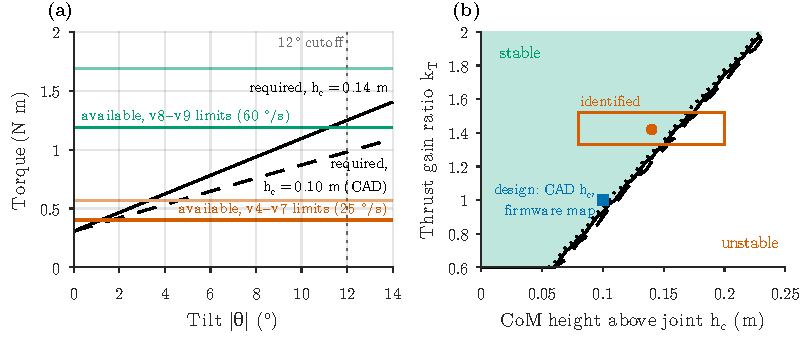
\includegraphics{figures/fig_drone_stability.pdf}
  \caption{Octocopter attitude loop. (a) Gravity torque required to hold a tilt (identified and CAD values of $h_c$) and available torque under angular-rate saturation \eqref{eq:tauavail}, for bench and flight limits; thick lines $k_T=1$, thin lines $k_T=1.42$. (b) Stability region of the full linear model in the $(h_c,k_T)$ plane; boundaries are drawn for $J=0.12$ (solid), 0.09 (dashed), and \SI{0.15}{\kilo\gram\metre\squared} (dotted). The rectangle marks the identified uncertainty and the square marks the design point (CAD $h_c$, firmware map).}
  \label{fig:dronestab}
\end{figure}

\subsubsection{Ball and plate}
\label{sec:ballcontrol}

\paragraph{Control law}
For each axis and each received camera frame, the ESP32-S3 computes
\begin{equation}
  u=u_n+\sat_{\pm220}\Big(k_p\,e+k_i\!\int\!e\,\dd t-k_d\,\hat v\Big),\qquad e=-x_b,
  \label{eq:ballpid}
\end{equation}
with velocity $\hat v$ from \eqref{eq:lsvel} computed by the Pi. The firmware works in \SI{3}{\milli\metre} units; in SI-consistent units, the gains $(1.5;\ 0.8;\ 4.5)$ become $k_p=\SI{0.50}{\micro\second\per\milli\metre}$, $k_i=\SI{0.27}{\micro\second\per\milli\metre\per\second}$, and $k_d=\SI{1.5}{\micro\second\per\milli\metre\second}$. Neutral pulse widths are $u_n=(1386;\ 1392)$\,\si{\micro\second}, the integral is clamped at 90\% of the output range, and the backlash from Section~\ref{sec:linkage} is added with a \SI{30}{\micro\second} ramp.

\paragraph{Discrete-time stability analysis}
Because the derivative acts through an FIR filter and the loop contains several pure delays (frame exposure and transfer, image processing, the \SI{50}{\hertz} servo frame, and analog-servo dead time), the loop was analyzed in discrete time at the camera period $h$: plant \eqref{eq:balltf} with a servo lag $\tau_s=\SI{50}{\milli\second}$ was discretized with a zero-order hold, total delay $T$ was represented by $T/h$ unit delays, the derivative used the exact FIR \eqref{eq:lsvel}, the integral used forward Euler, and stability was decided from the roots of the closed-loop characteristic polynomial. Figure~\ref{fig:ballstab}a shows the largest stable $k_d$ (in firmware units) versus $T$ for several plant gains. At the CAD gain $K_b=6.0$, the nominal $k_d=4.5$ is stable only if $T\lesssim\SI{40}{\milli\second}$---less than the sum of frame, processing, \SI{50}{\hertz} servo-frame, and servo dead-time delays. On the bench with rotors off, $k_d=4.5$ was stable and $k_d=6$ was unstable; for plausible delays ($T=$ 60--\SI{180}{\milli\second}), the model reproduces both observations only with an effective gain $K_{b,\mathrm{eff}}=3.5$--4.9 (58--82\% of the CAD value), where higher gains correspond to shorter delays. This reduction agrees with linkage backlash, whose describing function lowers small-signal gain, and with a direct regression of ball acceleration on logged servo pulses, which gives 2.5 and 4.9 for the $x$ and $y$ axes ($R^2=0.29$ and 0.45, limited by the 20\,Hz pulse logging rate). At $K_{b,\mathrm{eff}}=4.2$ and $T=\SI{0.10}{\second}$, the closed loop has a lightly damped fast mode at \SI{1.3}{\hertz} ($\zeta=0.06$), the signature of operating near the delay limit, and a slow integral mode at \SI{0.064}{\hertz} ($\zeta=0.37$, \SI{16}{\second} period).

\begin{figure}[!htbp]
  \centering
  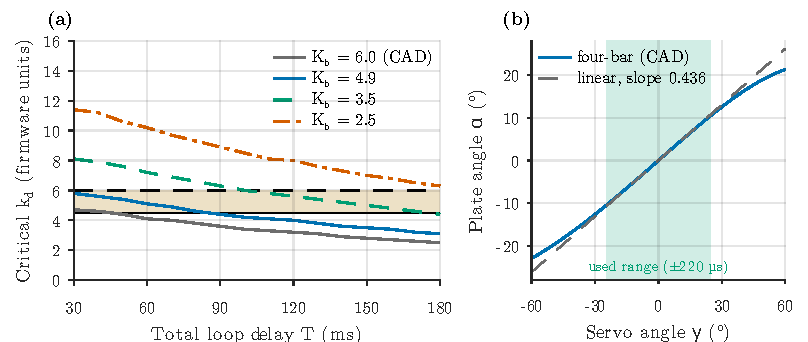
\includegraphics{figures/fig_ball_stability.pdf}
  \caption{Ball and plate. (a) Largest stable derivative gain (firmware units, $k_p=1.5$, $k_i=0.8$) versus total loop delay for four plant gains; the shaded band is bounded by the gain that was stable on the bench ($k_d=4.5$, solid line) and the one that was unstable ($k_d=6$, dashed). (b) Plate angle versus servo angle from the closed-form four-bar solution \eqref{eq:freud} and its linearization.}
  \label{fig:ballstab}
\end{figure}

\subsubsection{Mobile base}
\label{sec:basecontrol}
Each wheel runs a velocity PI loop with conditional integration (the integral freezes when the output saturates at 0 or 100\% duty cycle) using \SI{1}{\kilo\hertz} PWM. Go-to-goal mode uses the polar error $\rho=\|\vect p_g-\vect p\|$, $e_\psi=\operatorname{atan2}(\Delta y,\Delta x)-\psi$, whose kinematics follow from \eqref{eq:diff}: $\dot\rho=-v\cos e_\psi$, $\dot e_\psi=-\omega+(v/\rho)\sin e_\psi$. The law sets $\omega=\sat_{0.2}(1.2e_\psi)$, with $v=0$ while $|e_\psi|>\SI{0.2}{\radian}$ and $v=\min\{0.05;\ \max(0.025;\ 0.8\rho)\}$\,m/s otherwise, stopping once $\rho<\SI{2}{\centi\metre}$. Because no smooth time-invariant feedback can stabilize the full pose of a unicycle \cite{brockett1983}, the law regulates position only; convergence follows from elementary bounds. During the turning phase, $|e_\psi|$ decreases at no less than \SI{0.2}{\radian\per\second} until $|e_\psi|\le0.2$. During the approach phase, $\dot\rho\le-0.025\cos0.2<0$, and $V=e_\psi^2/2$ satisfies $\dot V\le-(\omega/e_\psi-v/\rho)\,e_\psi^2$ with $\omega/e_\psi\ge1$ and $v/\rho\le0.8$ for $\rho\ge\SI{3.1}{\centi\metre}$, so $|e_\psi|$ does not grow and the robot reaches the target tolerance in finite time after at most one turning phase.

\subsubsection{Octocopter altitude and heading (firmware v11)}
\label{sec:altura}
\paragraph{Heading on the base} The octocopter operates independently and receives no data from the base. At idle ($\le\SI{1400}{\micro\second}$), while mounted on the base, it holds its startup heading within a $\pm\SI{20}{\degree}$ \emph{sliding window}. If a base turn drags it past that limit, the reference slides with it instead of cutting the motors. It therefore does not fight the spherical joint during a \SI{360}{\degree} turn, and when the base stops it settles with at most a \SI{20}{\degree} offset. A safety cutoff remains active at \SI{120}{\degree\per\second}. Above \SI{1400}{\micro\second}, v9 behavior is retained: fixed heading hold with cutoffs at \SI{20}{\degree} and \SI{35}{\degree\per\second}. Under v9, base turns ended in the \SI{20}{\degree} cutoff.

\paragraph{Altitude measurement} The VL53L0X produced no valid readings during the 20 November flights. \SI{80}{\percent} of readings returned code~2 (\emph{signal fail}): the return signal from the laboratory floor (0.06--\SI{0.3}{MCPS}) fell below ambient infrared light (0.7--\SI{0.99}{MCPS}). Four measures were applied:
\begin{enumerate}[label=(\roman*)]
  \item a matte white \emph{target} (an A4 sheet) fixed to the base beneath the sensor, boosting signal return by a factor of 2 to 10; mounted on the base, the laser measures module position along the vertical guide---the variable of interest---independent of the floor or ramp;
  \item the sensor's long-range profile, with a \SI{0.05}{MCPS} signal limit, up to \SI{60}{\milli\metre} sigma, and \SI{66}{\milli\second} per reading;
  \item a three-reading median filter rejecting jumps larger than \SI{60}{\milli\metre};
  \item a linear ruler calibration at two guide heights: $d=0.930\,d_m-\SI{36.5}{\milli\metre}$.
\end{enumerate}
Accepted readings rose from \SI{0}{\percent} to nearly \SI{100}{\percent}, yielding 317--\SI{334}{\milli\metre} against \SI{330}{\milli\metre} measured with a ruler.

\paragraph{Sensor lever-arm correction} The laser sits on arm~8 ($+x$) at a horizontal distance $r_s$ from the spherical joint axis. When the module pitches by $\theta$ (positive nose-down, $+x$ downward in the FLU convention) or rolls by $\phi$, its tip moves vertically by $r_s\sin\theta$, altering the measured distance $d$ even when the spherical joint does not move along the guide. The axis height is
\begin{equation}
  z=d\cos\phi\cos\theta+r_s\sin\theta ,
  \label{eq:brazo}
\end{equation}
which feeds the filter. With $r_s=\SI{0.20}{\metre}$ (measured), a \SI{2}{\degree} pitch oscillation produces an apparent \SI{7}{\milli\metre} height shift without correction ($0.20\sin 2^\circ\approx\SI{7.0}{\milli\metre}$); the firmware applies \eqref{eq:brazo} to every reading before filtering. For the same reason, the IMU accelerometer, also on arm~8, measures the tangential and centripetal accelerations of module rotation ($\dot{\vect\omega}\times\vect r_s+\vect\omega\times(\vect\omega\times\vect r_s)$). At hover angular rates below \SI{10}{\degree\per\second}, this term is smaller than \SI{0.05}{\metre\per\second\squared} and falls within the filter's process noise.

\paragraph{Altitude Kalman filter} Altitude is estimated by fusing the laser with the accelerometer. The state is $\vect x=[z,\ v,\ b]^{\top}$, where $z$ is the distance to the target, $v$ is vertical velocity, and $b$ is vertical accelerometer bias. Prediction runs at the IMU rate using world-frame vertical acceleration from the \SI{10}{\hertz}-filtered accelerometer and estimated attitude:
\begin{equation}
  \begin{gathered}
    a_z=\big(-\sin\theta\,a_x+\sin\phi\cos\theta\,a_y+\cos\phi\cos\theta\,a_z^{b}\big)g-g,\\
    z_{k+1}=z_k+v_k\Delta t+\tfrac12(a_z-b_k)\Delta t^2,\quad
    v_{k+1}=v_k+(a_z-b_k)\Delta t,\quad b_{k+1}=b_k .
  \end{gathered}
  \label{eq:kfz}
\end{equation}
Process noise is $\sigma_a=\SI{0.6}{\metre\per\second\squared}$ on acceleration and $\sigma_b=\SI{0.02}{\metre\per\second\squared}/\sqrt{\mathrm{s}}$ on bias. Each accepted laser reading updates the state with $R=(\SI{52}{\milli\metre})^2$, the dispersion measured over the floor. Updates pass through a $3\sigma$ gate, and the filter resynchronizes after five consecutive rejections. In simulation with measured noise, altitude error drops from \SI{73}{\milli\metre} (raw laser) to 33--\SI{52}{\milli\metre}. On the bench with the target, filter uncertainty is about \SI{23}{\milli\metre}.

\paragraph{Cascaded altitude control} The vertical plant is a double integrator, compounded by motor lag (\SI{70}{\milli\second}), sensor delay (\SI{66}{\milli\second} plus median filtering), and dry guide friction that causes stick--slip jumps. A single PID on altitude therefore oscillates. A cascade is used instead:
\begin{equation}
  \begin{gathered}
    v_{\mathrm{ref}}=\mathrm{sat}_{\pm\SI{40}{\milli\metre\per\second}}\!\big(k_z(z_{\mathrm{ref}}-\hat z)\big),\\
    \Delta u=\mathrm{sat}_{\pm\SI{60}{\micro\second}}\!\Big(k_{vp}(v_{\mathrm{ref}}-\hat v)+k_{vi}\!\int(v_{\mathrm{ref}}-\hat v)\,dt\Big),
  \end{gathered}
  \label{eq:cascada}
\end{equation}
with $k_z=\SI{1.5}{\per\second}$, $k_{vp}=\SI{0.18}{\micro\second\per(\milli\metre\per\second)}$, $k_{vi}=\SI{0.35}{\micro\second\per\milli\metre}$, and integrator anti-windup. The reference $z_{\mathrm{ref}}$ follows the target along a \SI{20}{\milli\metre\per\second} ramp; the \emph{Subir} (Up) and \emph{Bajar} (Down) commands step it by $\pm\SI{20}{\milli\metre}$. The inner loop uses velocity from the Kalman filter, avoiding the lag of differentiating laser readings so the module brakes before arrival. Its integrator compensates for battery voltage sag and friction.

In simulation with Coulomb friction and stick--slip in the guide, peak-to-peak oscillation drops from 13--\SI{46}{\milli\metre} with PID to 4--\SI{12}{\milli\metre} with the cascade. Altitude hold activates via \emph{Mantener} (Hold) only if filter uncertainty is below \SI{30}{\milli\metre}; otherwise the collective stays fixed. Flight validation remains pending.

\subsection{Coupled model and disturbance propagation}
\label{sec:coupling}

Combining the linearized octocopter \eqref{eq:pitchlin} closed with \eqref{eq:cascade} and the ball \eqref{eq:balllinx} closed with \eqref{eq:ballpid} gives the propagation from base acceleration to ball position:
\begin{gather}
  X_b(s)=\frac{S_b(s)}{s^2}\Big\{\gamma_b\Big[\big(g-(h_P+\kappa)s^2\big)\,T_{\theta A}(s)-1\Big]A_{J,x}(s)+D_b(s)\Big\}, \label{eq:propag}\\
  T_{\theta A}(s)=\frac{-m h_c\,P(s)}{1+L_D(s)}, \notag
\end{gather}
where $P(s)=1/(J_ys^2-mgh_c)$, $L_D$ is the open-loop transfer function of the attitude cascade, $S_b=1/(1+L_b)$ is the sensitivity of the ball loop, and $D_b$ gathers all disturbances acting directly on the ball (airflow, vibration, backlash). Figure~\ref{fig:transm} evaluates \eqref{eq:propag}. Three findings stand out.

\begin{enumerate}[label=(\roman*)]
  \item \textbf{Rotation and slope are benign.} Centripetal acceleration of the spherical joint during the course-guide turns (wheel speeds up to \SI{0.10}{\metre\per\second}) is at most \SI{0.024}{\metre\per\second\squared} about the axle midpoint and \SI{0.015}{\metre\per\second\squared} about one wheel, equivalent to less than \SI{0.15}{\degree} of plate tilt; slope does not enter the ball equation \eqref{eq:tilt} at all. Only ramp transitions and base starts and stops produce significant accelerations.
  \item \textbf{The octocopter amplifies slow base accelerations.} Because its net stiffness \eqref{eq:stiff} is small, the module responds to base accelerations near its slow mode (0.2--\SI{0.3}{\hertz}) with tilts of several degrees per m/s$^2$ (Fig.~\ref{fig:transm}b), and between 0.1 and \SI{1}{\hertz} this path dominates over the direct path to the ball (Fig.~\ref{fig:transm}c). This agrees with the tilt cutoffs at the ramp edges in the integrated tests. It is the dynamic cost of a drone compared to a rigid gimbal (Section~\ref{sec:porquedron}).
  \item \textbf{Attitude motion is not the main source of ball error.} Filtering the measured octocopter attitude at idle (bench log, RMS 0.23--\SI{0.37}{\degree}) through $X_b/\Theta$ predicts a ball RMS of only 1.7--\SI{2.1}{\milli\metre}, whereas measured RMS with rotors spinning and base stationary is 16--\SI{21}{\milli\metre} in $x$ and 10--\SI{12}{\milli\metre} in $y$. Over 90\% of the measured variance lies below \SI{0.3}{\hertz}, with spectral peaks between 0.02 and \SI{0.05}{\hertz} (20--45\,s periods), the timescale of the ball loop's slow integral mode (\SI{0.064}{\hertz}). The dominant disturbance is therefore a slowly varying load acting directly on the ball ($D_b$): rotor airflow over the plate, vibration-induced drift, and backlash, which pulled the ball toward $(-x,-y)$ during tests. Only integral action rejects it, and its bandwidth is limited by delay.
\end{enumerate}

\begin{figure}[!htbp]
  \centering
  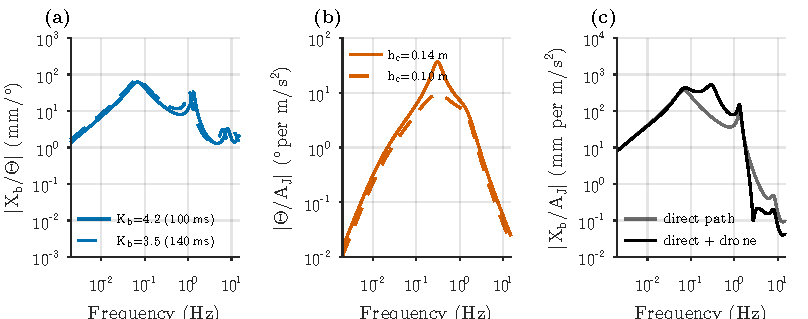
\includegraphics{figures/fig_transmissibility.pdf}
  \caption{Disturbance propagation predicted by \eqref{eq:propag} (hover gains, $k_T=1.42$). (a) Ball displacement per degree of octocopter tilt with the ball loop closed. (b) Octocopter tilt per unit base acceleration. (c) Ball displacement per unit base acceleration, via the direct path and through the octocopter.}
  \label{fig:transm}
\end{figure}

\subsection{Fundamental limitations and design implications}
\label{sec:limits_fund}
The model also bounds what any controller can achieve with the current hardware \cite{skogestad2005}.
\begin{itemize}
  \item \textbf{Octocopter.} An unstable pole $p$ demands a crossover above $\approx2p$, while an effective delay $\theta_e$ caps it at $\approx1/\theta_e$; robust stabilization requires roughly $p\,\theta_e<0.5$. With $p=\SI{6.1}{\radian\per\second}$ and $\theta_e\approx\tau_m+T_a=\SI{0.09}{\second}$, $p\theta_e=0.55$: attitude control on the spherical joint operates at the edge of this limit. The structural remedy is to lower the center of mass: with the batteries below the spherical joint ($h_c<0$), the module becomes a stable pendulum and the torque authority demanded by \eqref{eq:thetastar} decreases; low-mounted batteries would also improve tip-over stability on the ramp.
  \item \textbf{Ball and plate.} The right-half-plane zero $z_1=\SI{15.2}{\radian\per\second}$ limits crossover to $\approx z_1/2=\SI{7.6}{\radian\per\second}$, and the $\approx$\SI{0.1}{\second} delay limits it to $\approx\SI{10}{\radian\per\second}$; the PID operates at $K_{b,\mathrm{eff}}k_d\approx\SI{6}{\radian\per\second}$, near both bounds, explaining the ceiling on $k_d$. Faster ball control requires lower delay (\SI{333}{\hertz} digital servos, frame-synchronized servo updates) and smaller $\kappa$ (moving the plate surface closer to the universal joint center).
  \item \textbf{Mobile base.} Both the acceleration margin \eqref{eq:tip} and the octocopter's slow mode call for smooth (jerk-limited) base references; on a \SI{20}{\degree} slope, the thrust-free acceleration margin is only \SI{0.26}{\metre\per\second\squared}, rising to 0.7--\SI{1.0}{\metre\per\second\squared} when the rotors support 35--55\% of the module weight (Section~\ref{sec:porquedron}). Alternatives are low-mounted ballast or a lower aerial module.
  \item \textbf{Power.} Thrust margin drops with the square of battery voltage (Section~\ref{sec:bateria}); without voltage sensing and collective compensation, usable hover time is 3--\SI{7}{\minute} per LiPo pair.
\end{itemize}
